\setcounter{page}{2}

\section{Содержание задания}
Проект представляет собой создание карты города.
В проекте участвуют 16 разработчиков, бюджет проекта~---~50000 рублей, длительность проекта~---~6 месяцев.
Дата начала проекта~---~первый рабочий день марта текущего года.

Появление перегрузки для ресурса <<Системный аналитик>> связано с тем, что данный ресурс задействован при выполнении задач <<Анализ и построение структуры базы объектов>> и <<Анализ и проектирование ядра>>, сроки реализаций которых накладываются.

Появление перегрузки для ресурса <<Художник-дизайнер>> связано с тем, что данный ресурс задействован при выполнении задач <<Разработка дизайна руководства>> и <<Разработка дизайна сайта>>, сроки реализаций которых накладываются.

Появление перегрузки для ресурса <<Технический писатель>> связано с тем, что данный ресурс задействован при выполнении задач <<Написание руководства пользователя>> и <<Создание справочной системы>>, сроки реализаций которых накладываются.

Устранить перегрузки возможно следующими способами:
\begin{itemize}[label=---]
	\item изменить календарь работы ресурса;
	\item назначить ресурс на неполный день;
	\item добавить ресурсу время задержек;
	\item применить автоматическое выравнивание.
\end{itemize}

\section{Задание 1}

В проекте перегружено несколько ресурсов, поэтому для устранения перегрузок необходимо использовать автоматическое выравнивание.
Параметры выравнивания представлены на рисунке~\ref{fig:screen1}.
Выравнивание должно выполняться автоматически и во всем проекте. Во избежание очистки данных предыдущего выравнивания перед новым выравниванием необходимо убрать соответствующий флажок.

\begin{figure}[H]
	\centering
	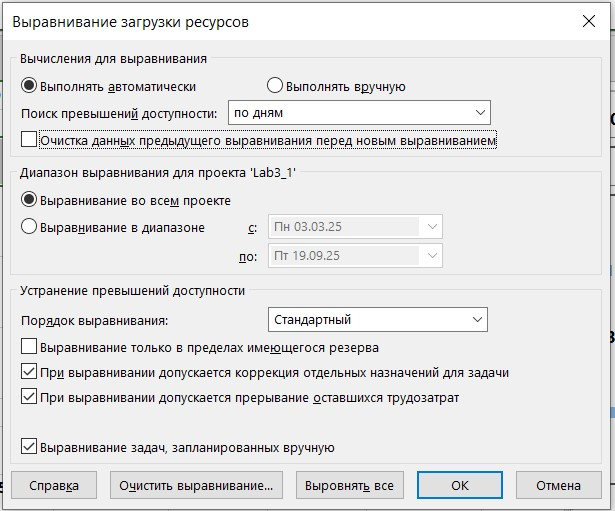
\includegraphics[width=0.9\textwidth]{img/task1/screen1.jpg}
	\caption{Параметры выравнивания}
	\label{fig:screen1}
\end{figure}

После применения автоматического выравнивания бюджет проекта сократился на 2 рубля за счет смещения вехи <<Построение базы объектов>> с 03.03 на 24.03, за счет чего работа команды не попала на предпраздничный укороченный день 07.03.
Окончание проекта сместилось с 19.09 на 23.09, а трудозатраты снизились с 9419 часов до 9418 часов.

Сведения для проекта после выравнивания отражены на рисунке~\ref{fig:screen2}.

\begin{figure}[H]
	\centering
	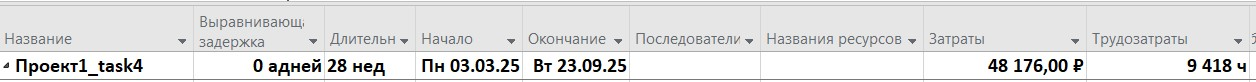
\includegraphics[width=0.9\textwidth]{img/task1/screen2.jpg}
	\caption{Сведения о проекте после выравнивания}
	\label{fig:screen2}
\end{figure}

Диаграмма Ганта после выравнивания приведена на рисунке~\ref{fig:screen3}.

\begin{figure}[H]
	\centering
	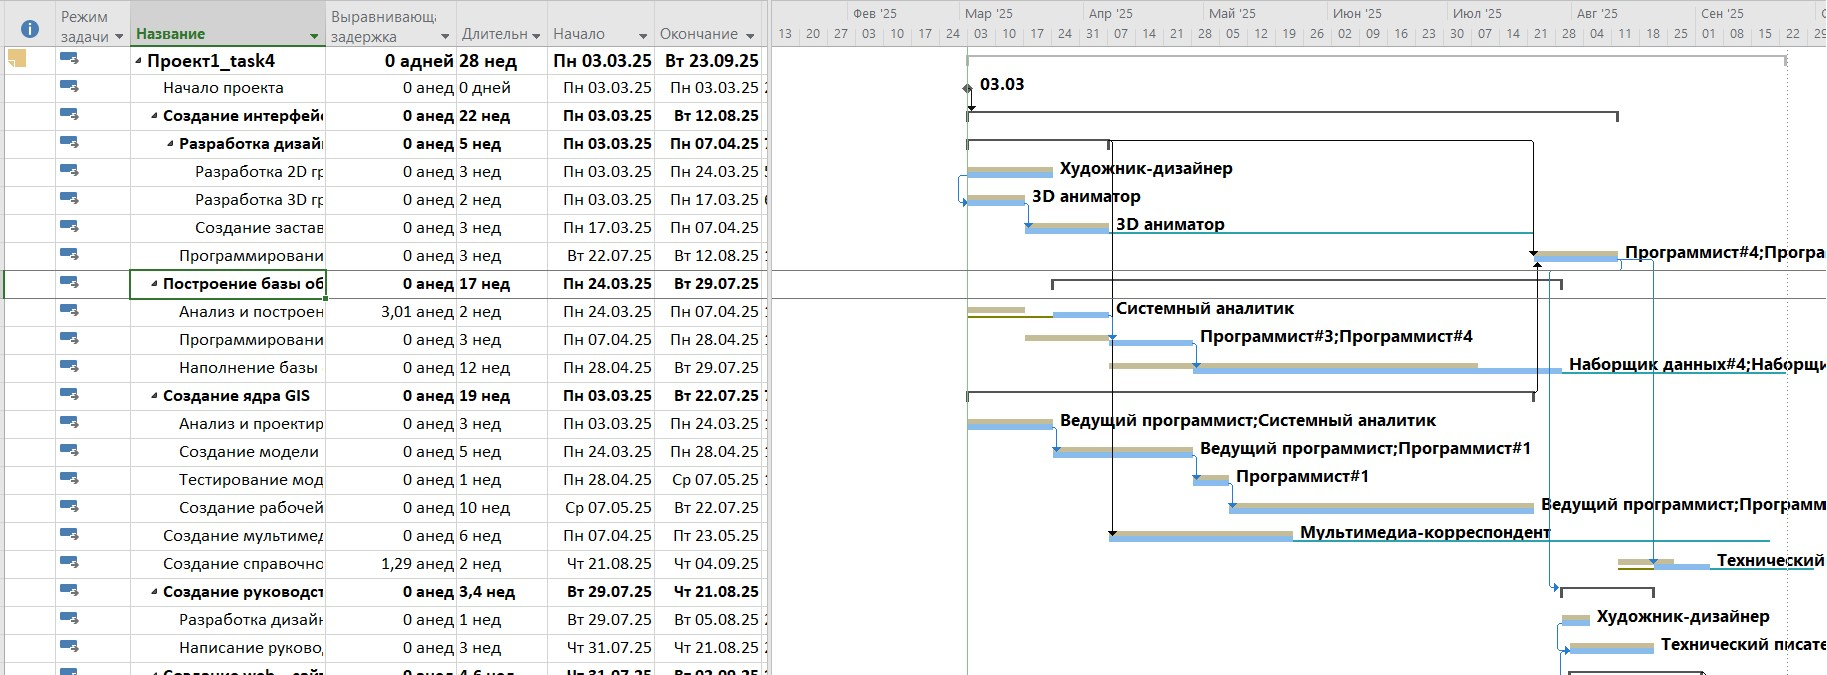
\includegraphics[width=0.9\textwidth]{img/task1/screen3.jpg}
	\caption{Диаграмма Ганта после выравнивания}
	\label{fig:screen3}
\end{figure}

Перегрузки ресурса <<Системный аналитик>> устранены за счет ввода задержки для задачи <<Анализ и построение структуры базы объектов>>.
Срок выполнения задачи до выравнивания~---~с 03.03 до 17.03, после выравнивания~---~с 24.03 до 07.04.
Задаче <<Анализ и проектирование ядра>> не могут быть добавлены задержки, так как она входит в критический путь.
Задачам критического пути нельзя добавить задержки, так как они влияют на дату окончания проекта.
Данная задержка приведена на рисунках~\ref{fig:screen4} и~\ref{fig:screen5}.

\begin{figure}[H]
	\centering
	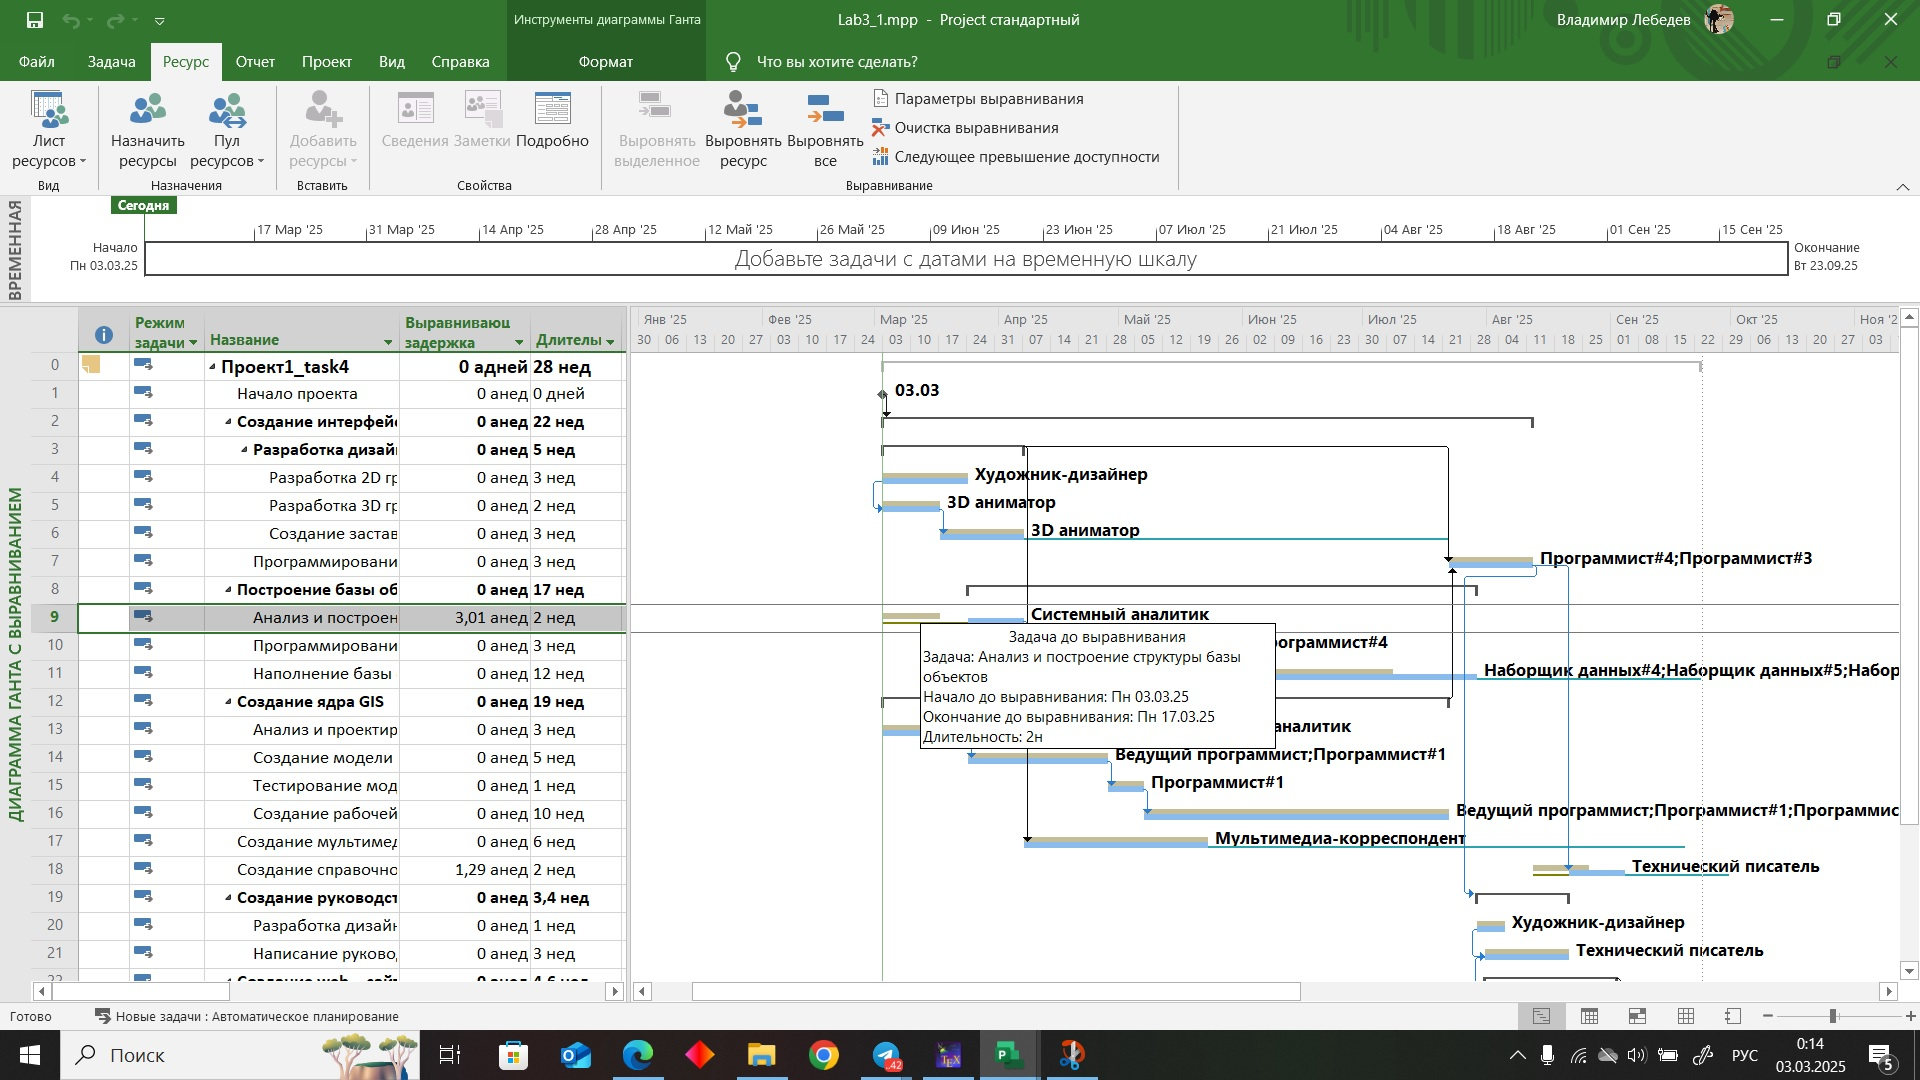
\includegraphics[width=0.9\textwidth]{img/task1/screen4.jpg}
	\caption{<<Анализ и построение структуры базы объектов>> до выравнивания}
	\label{fig:screen4}
\end{figure}

\begin{figure}[H]
	\centering
	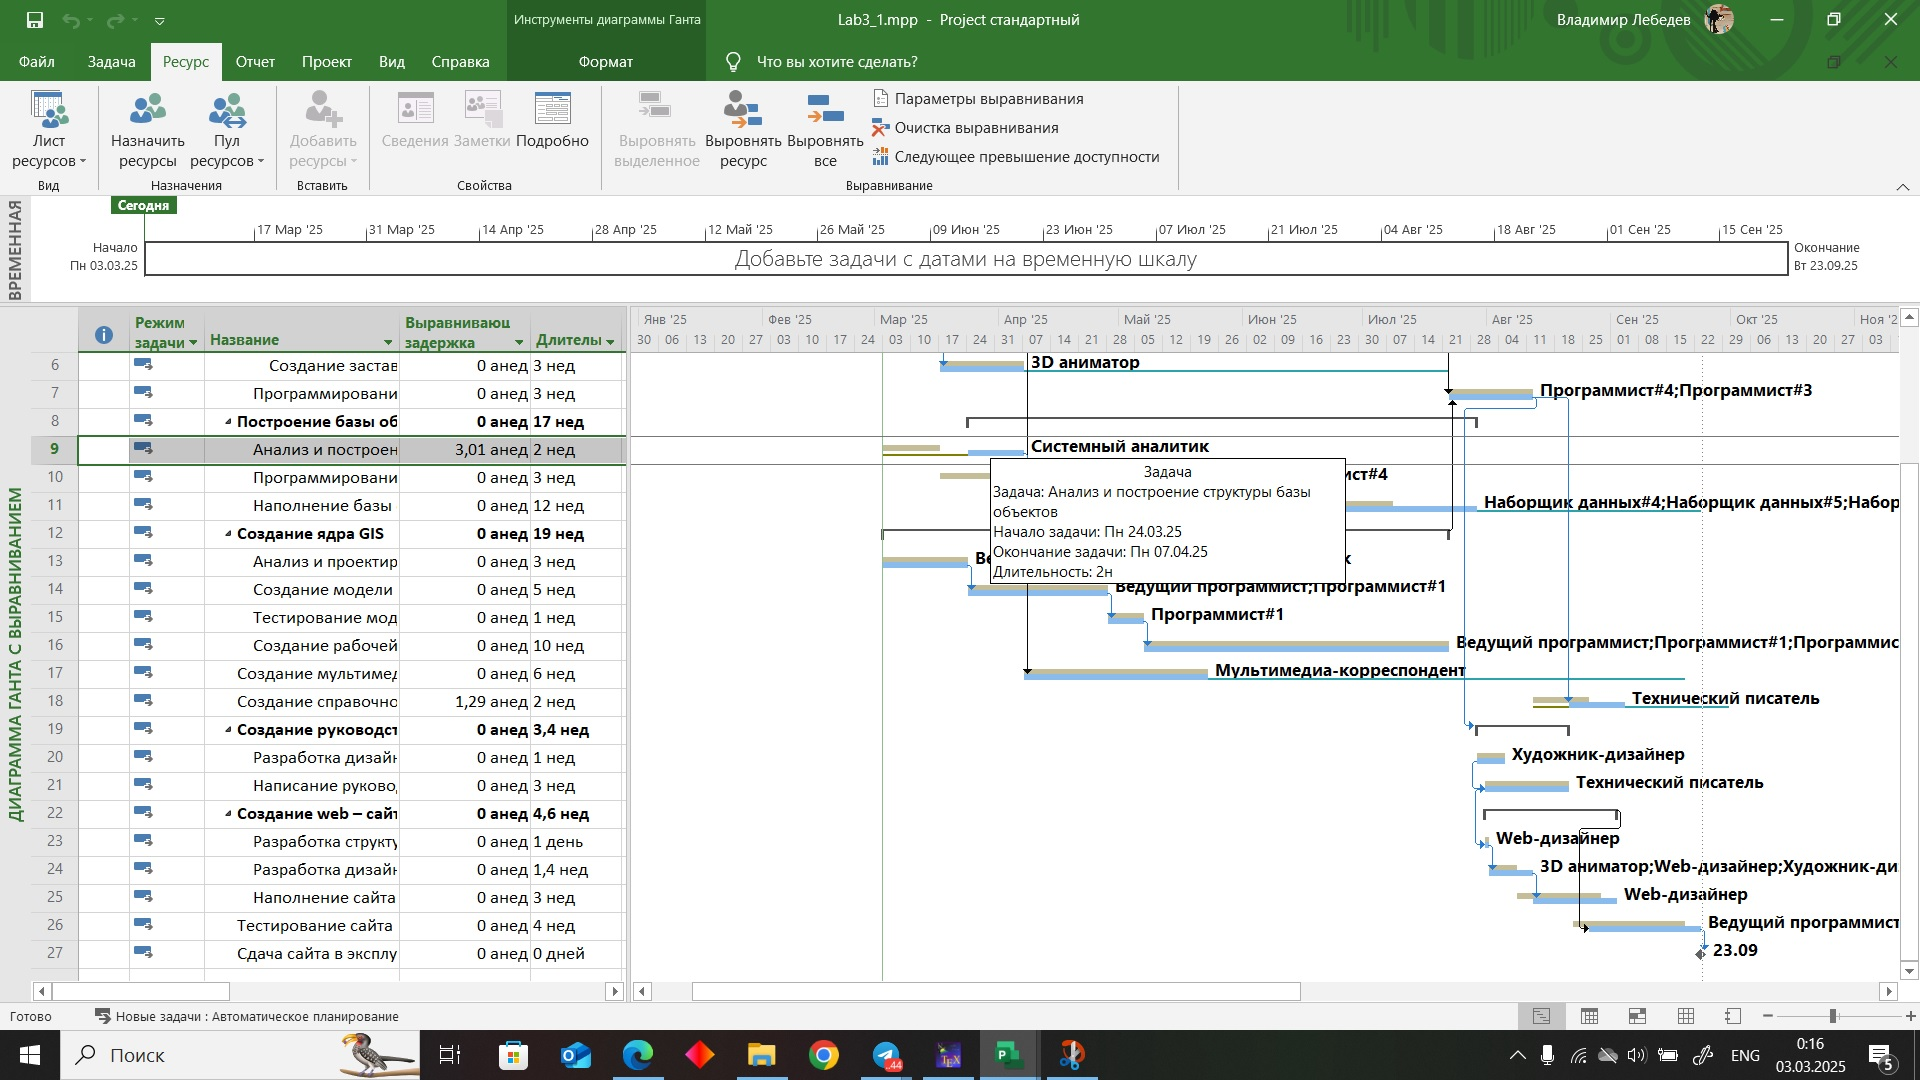
\includegraphics[width=0.9\textwidth]{img/task1/screen5.jpg}
	\caption{<<Анализ и построение структуры базы объектов>> после выравнивания}
	\label{fig:screen5}
\end{figure}

Перегрузки ресурса <<Технический писатель>> устранены за счет ввода задержки для задачи <<Создание справочной системы>>.
Срок выполнения задачи до выравнивания~---~с 12.08 до 26.08, после выравнивания~---~с 21.08 до 04.09.
Задаче <<Написание руководства пользователя>> не могут быть добавлены задержки, так как она входит в критический путь.
Данная задержка приведена на рисунках~\ref{fig:screen6} и~\ref{fig:screen7}.

\begin{figure}[H]
	\centering
	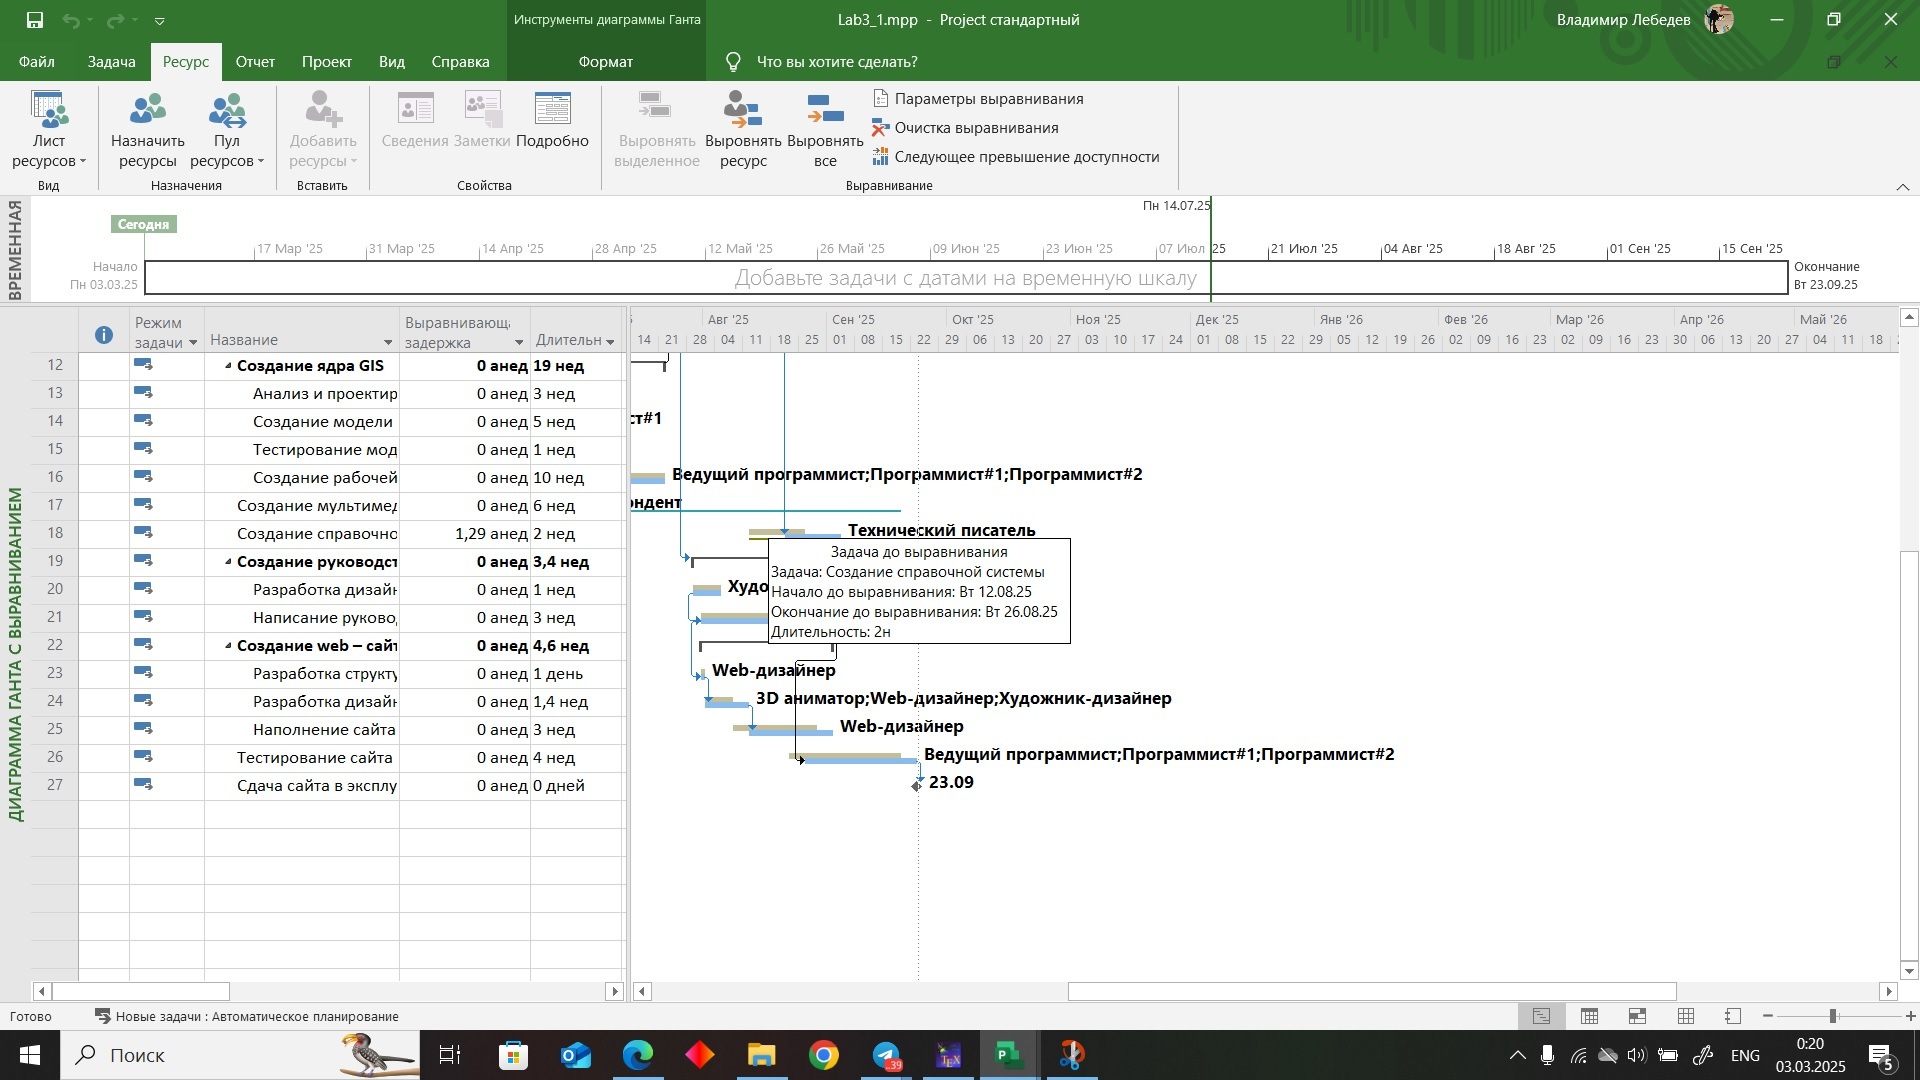
\includegraphics[width=0.9\textwidth]{img/task1/screen6.jpg}
	\caption{<<Создание справочной системы>> до выравнивания}
	\label{fig:screen6}
\end{figure}

\begin{figure}[H]
	\centering
	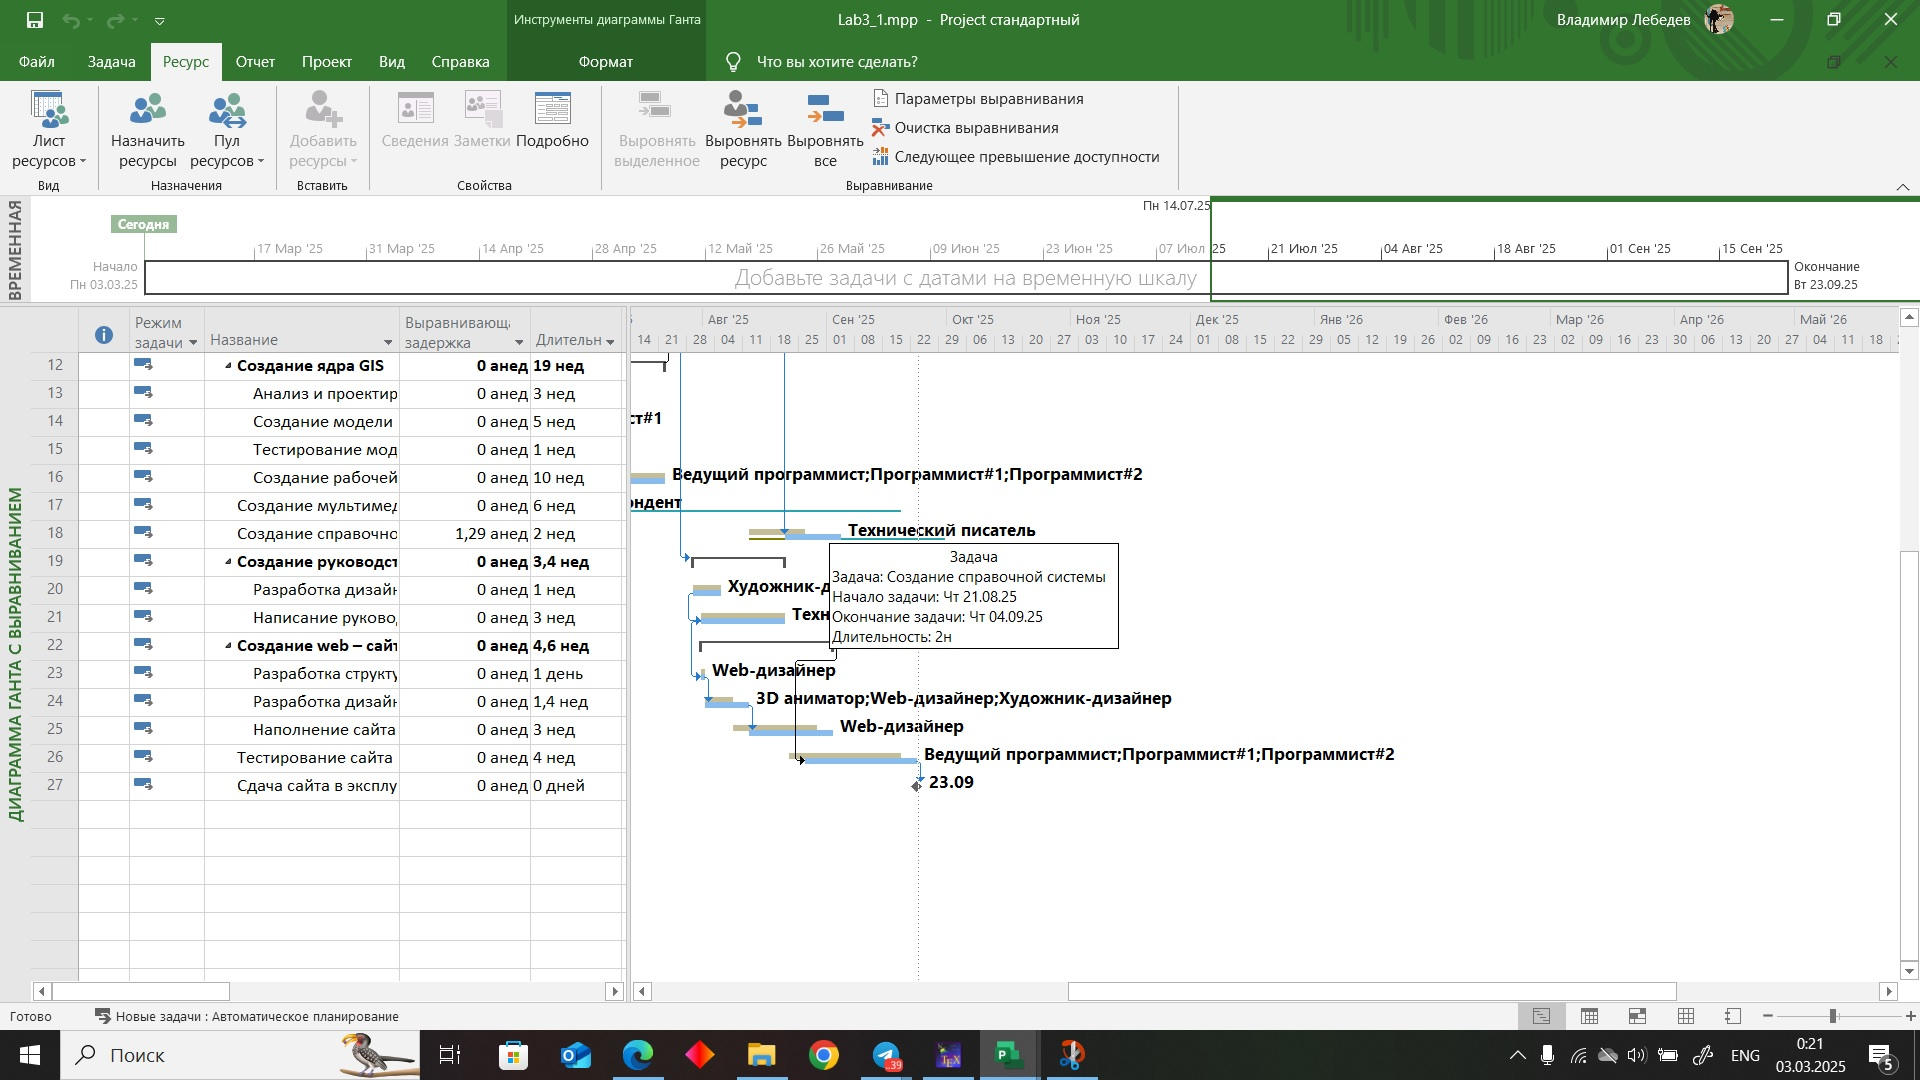
\includegraphics[width=0.9\textwidth]{img/task1/screen7.jpg}
	\caption{<<Создание справочной системы>> после выравнивания}
	\label{fig:screen7}
\end{figure}

Перегрузка ресурса <<Художник-дизайнер>> устранена путем введения задержки на 4 дня для него в рамках задачи <<Разработка дизайна сайта>>, что отражено на рисунке~\ref{fig:screen8}.
Задачи <<Разработка дизайна сайта>> и <<Разработка дизайна руководства>>, в которых участвует художник-дизайнер, входят в критический путь, из-за чего им не могут быть добавлены задержки.
Поэтому задержки добавлены для начала работы художника-дизайнера в задаче <<Разработка дизайна сайта>>, что привело к увеличению срока проекта на 4 дня.

\begin{figure}[H]
	\centering
	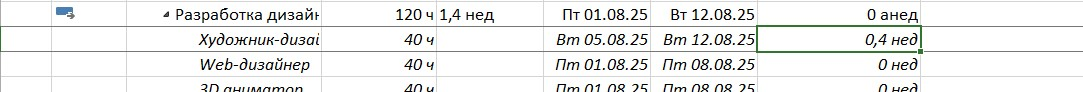
\includegraphics[width=0.9\textwidth]{img/task1/screen8.jpg}
	\caption{Задержка для ресурса <<Художник-дизайнер>> в рамках <<Разработки дизайна сайта>>}
	\label{fig:screen8}
\end{figure}

\section{Задание 2}

Необходимо добавить задачу <<Совещание>>, которая будет повторяться каждую среду с 10:00 до 11:00.
В совещании задействованы все специалисты кроме наборщиков и программистов №1-4.
Настройка повторяющегося события <<Совещание>> приведена на рисунке~\ref{fig:screen2_1}.

\begin{figure}[H]
	\centering
	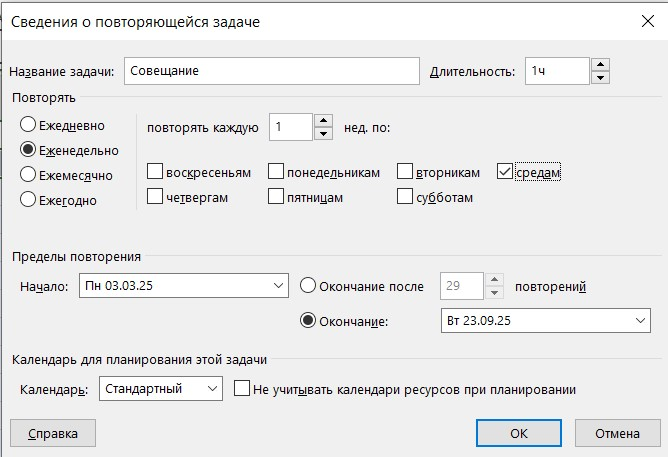
\includegraphics[width=0.9\textwidth]{img/task2/screen1.jpg}
	\caption{Настройка повторяющегося события <<Совещание>>}
	\label{fig:screen2_1}
\end{figure}

Назначение ресурсов, трудозатраты и затраты на ресурсы во время совещания, а также обновленные сроки проекта приведены на рисунке~\ref{fig:screen2_2}.
Трудозатраты на одно совещание составили 7 часов, затраты~---~691 рубль.
Суммарно на все совещания потрачено 203 часа трудозатрат и 20039 рублей.
Таким образом, окончание проекта сместилось с 19.09 на 26.09, бюджет проекта превысил заложенные 50000 рублей и составил 68219 рублей.
Перегрузка ресурсов была устранена автоматически.

\begin{figure}[H]
	\centering
	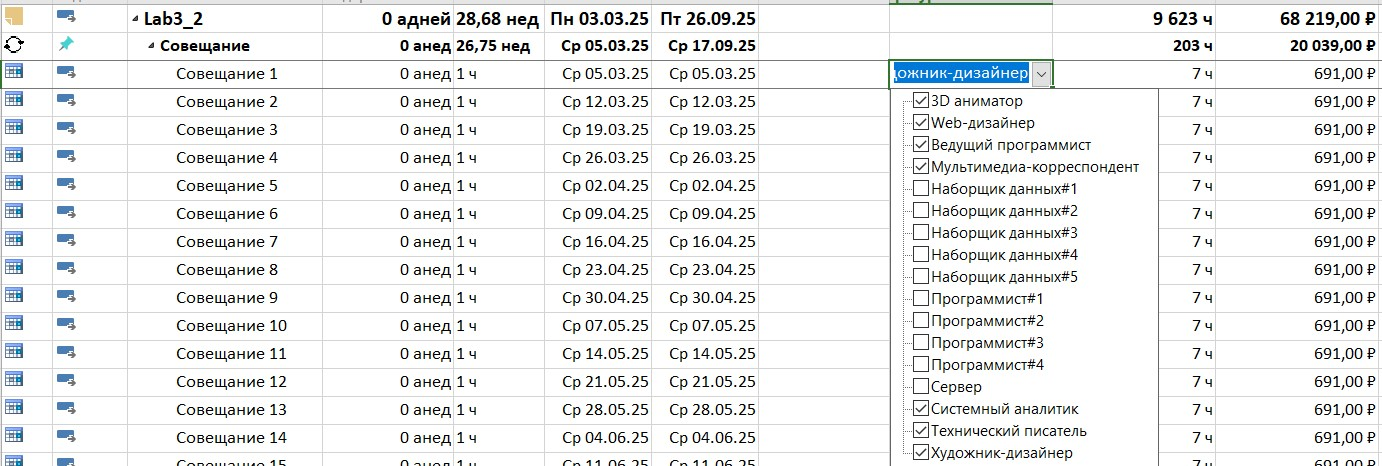
\includegraphics[width=0.9\textwidth]{img/task2/screen2.jpg}
	\caption{Изменения в проекте после добавления <<Совещания>>}
	\label{fig:screen2_2}
\end{figure}

Для всех человеческих ресурсов указаны затраты на использование, то есть дополнительные расходы, связанные с доставкой, установкой, наладкой оборудования для сотрудников, обучением персонала.
Эти затраты не следует учитывать в рамках <<Совещания>>.
Для этого необходимо ввести новую ставку, при которой затраты на использование равны нулю, что демонстрируется на рисунке~\ref{fig:screen2_3}.

\begin{figure}[H]
	\centering
	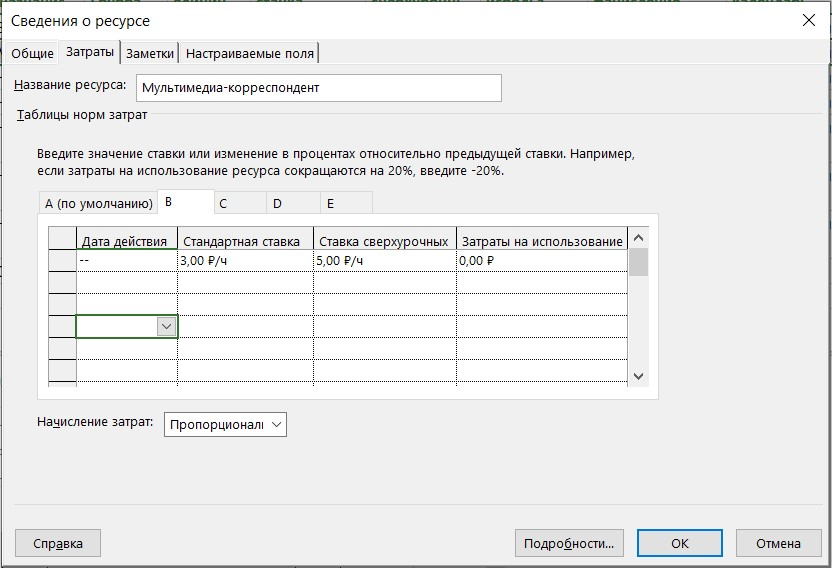
\includegraphics[width=0.9\textwidth]{img/task2/screen3.jpg}
	\caption{Добавление новой ставки для ресурса <<Мультимедиа-корреспондент>>}
	\label{fig:screen2_3}
\end{figure}

После добавления новой ставки необходимо выбрать ее для каждого ресурса, задействованного в <<Совещании>>.
Такая настройка, доступная в разделе <<Вид>> --- <<Использование задач>> --- <<Сведения о назначении>>, приведена на рисунке~\ref{fig:screen2_4}.

\begin{figure}[H]
	\centering
	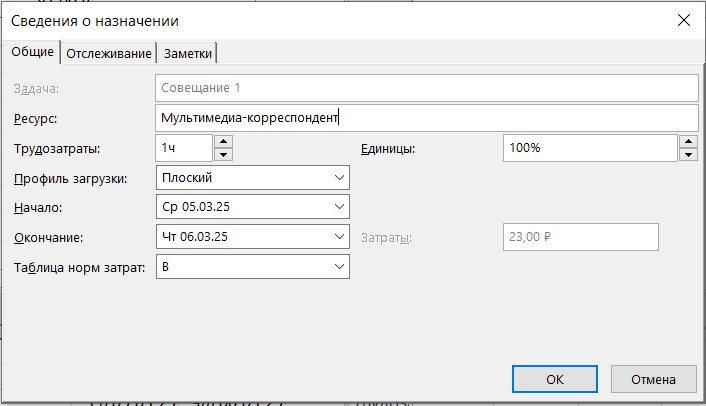
\includegraphics[width=0.9\textwidth]{img/task2/screen4.jpg}
	\caption{Смена ставки для ресурса}
	\label{fig:screen2_4}
\end{figure}

Затраты на одно совещание после смены ставки составили 61 рубль, на все совещания~---~1769 рублей, на весь проект~---~49949 рублей, что укладывается в бюджет в 50000 рублей.
Несмотря на введение новой ставки, на совещание все равно добавляются дополнительные трудозатраты, из-за чего бюджет проекта увеличился на 1769 рублей по сравнению с проектом в лабораторной работе №2, тем самым запас бюджета составляет 51 рубль.
Выравнивание выполнялось автоматически путем дробления задач.
Затраты после смены ставки приведены на рисунке~\ref{fig:screen2_5}.

\begin{figure}[H]
	\centering
	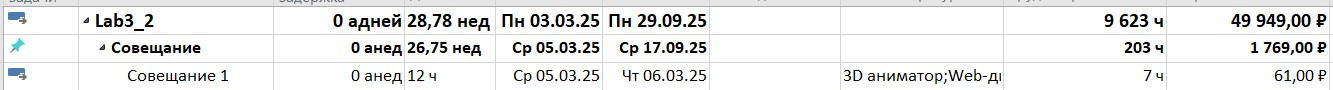
\includegraphics[width=0.9\textwidth]{img/task2/screen5.jpg}
	\caption{Затраты после смены ставки сотрудников}
	\label{fig:screen2_5}
\end{figure}

\section{Задание 3}

Критический путь проекта представлен на рисунке~\ref{fig:screen3_1}.

\begin{figure}[H]
	\centering
	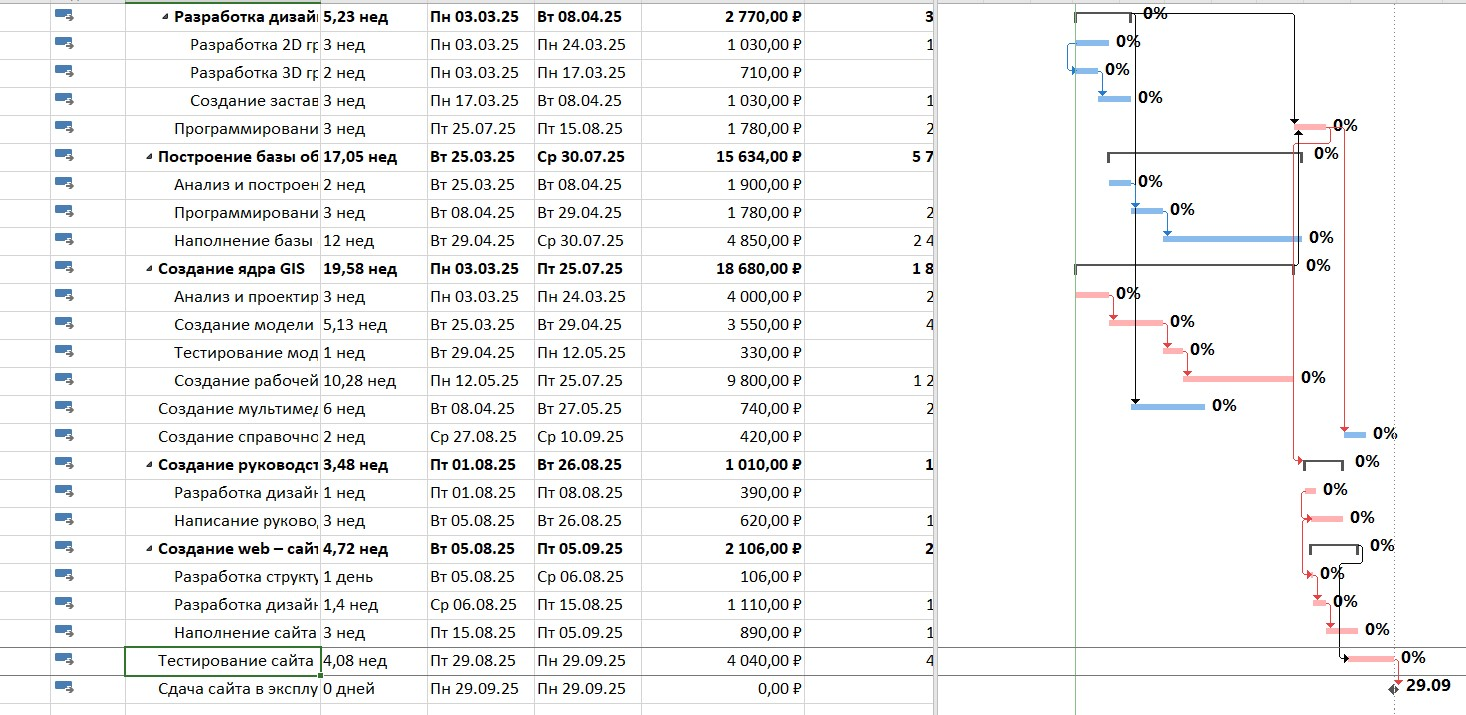
\includegraphics[width=0.9\textwidth]{img/task3/screen1.jpg}
	\caption{Критический путь проекта}
	\label{fig:screen3_1}
\end{figure}

Исходя из диаграммы Ганта с отслеживанием, критический путь состоит из задач <<Анализ и проектирование ядра>>, <<Создание модели>>, <<Тестирование модели>>, <<Создание рабочей версии ядра>>, <<Программирование интерфейса>>, <<Разработка дизайна руководства>>, <<Написание руководства пользователя>>, <<Наполнение сайта>> и <<Тестирование сайта>>.

Для оптимизации критического пути выполнены следующие действия:
\begin{itemize}[label=---]
	\item к ресурсам задачи <<Создание модели>> добавлен ресурс <<Программист №2>>;
	\item к ресурсам задачи <<Тестирование сайта>> добавлены ресурсы <<Программист №3>> и <<Программист №4>>;
	\item к ресурсам задачи <<Создание рабочей версии ядра>> добавлены ресурсы <<Программист №3>> и <<Программист №4>>.
\end{itemize}

К ресурсам задачи <<Создание модели>> не добавлены программисты №3-4, так как их добавление увеличивает затраты проекта.
Добавление ресурсов представлено на рисунке~\ref{fig:screen3_2}.
Так как задачи имеют фиксированные трудозатраты, при увеличении количества ресурсов уменьшается продолжительность задачи.
Окончание проекта сместилось на 12.08, то есть удалось сократить сроки проекта более, чем на месяц и уложиться в срок 6 месяцев.

\begin{figure}[H]
	\centering
	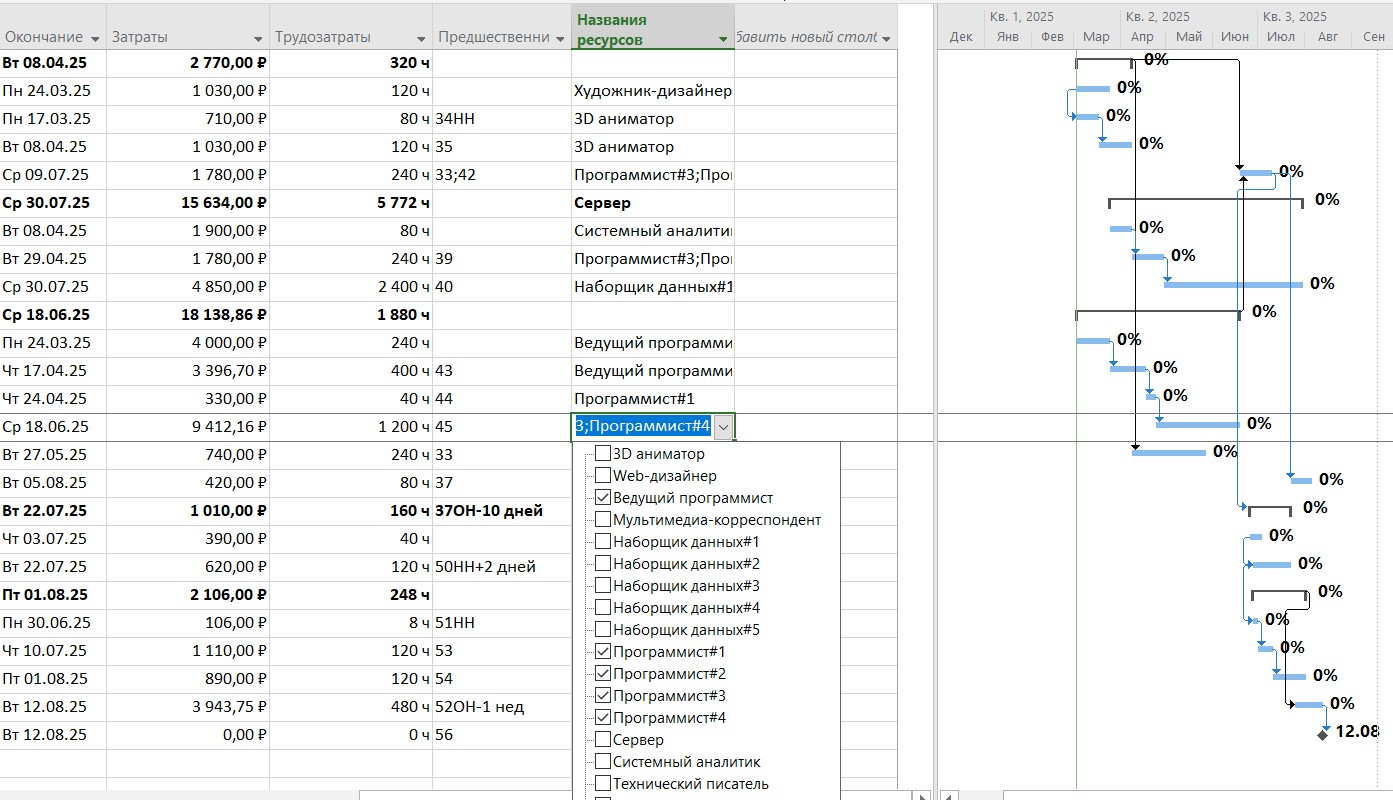
\includegraphics[width=0.9\textwidth]{img/task3/screen2.jpg}
	\caption{Добавление ресурсов}
	\label{fig:screen3_2}
\end{figure}

Так как дата окончания проекта изменилась, необходимо уменьшить число совещаний путем изменения даты окончания повторяющегося события <<Совещание>>, что продемонстрировано на рисунке~\ref{fig:screen3_3}.
Последнее совещание состоится 06.08.

\begin{figure}[H]
	\centering
	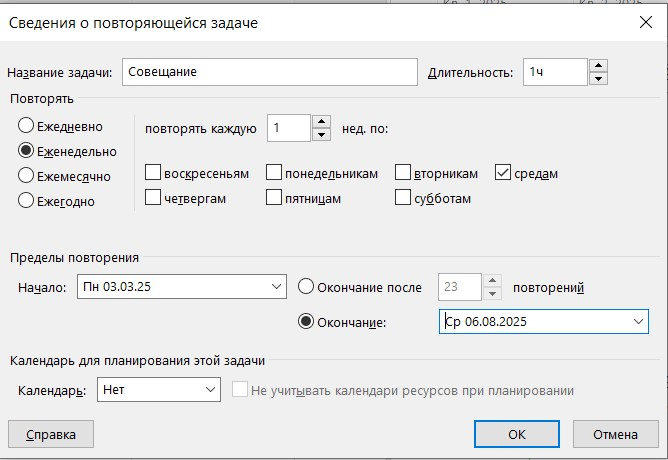
\includegraphics[width=0.9\textwidth]{img/task3/screen3.jpg}
	\caption{Изменение параметров повторяющегося события <<Совещание>>}
	\label{fig:screen3_3}
\end{figure}

Проект завершится 12.08 с затратами 48945 рублей, уложившись в срок 6 месяцев и бюджет 50000 рублей.
По сравнению с 
Информация о проекте и его статистика приведены на рисунках~\ref{fig:screen3_4} и~\ref{fig:screen3_9}.

\begin{figure}[H]
	\centering
	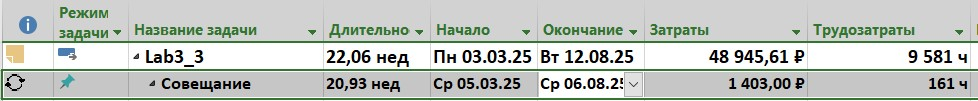
\includegraphics[width=0.9\textwidth]{img/task3/screen4.jpg}
	\caption{Информация о проекте}
	\label{fig:screen3_4}
\end{figure}

\begin{figure}[H]
	\centering
	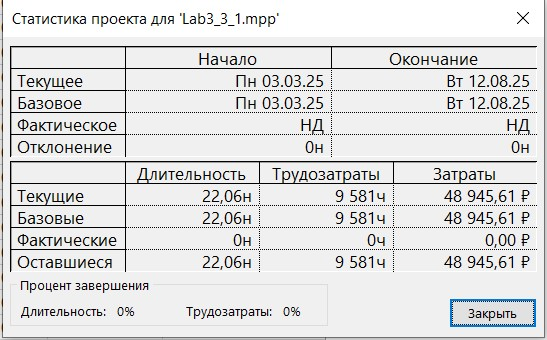
\includegraphics[width=0.9\textwidth]{img/task3/screen9.jpg}
	\caption{Статистика проекта}
	\label{fig:screen3_9}
\end{figure}

Затраты на группы ресурсов приведены на рисунке~\ref{fig:screen3_7}.

На рисунках~\ref{fig:screen3_5} и~\ref{fig:screen3_6} отображены диаграммы трудозатрат и затрат.

\begin{figure}[H]
	\centering
	
\includegraphics[width=0.9\textwidth]{img/task3/screen10.jpg}
	\caption{Затраты на группы ресурсов}
	\label{fig:screen3_7}
\end{figure}

\begin{figure}[H]
	\centering
	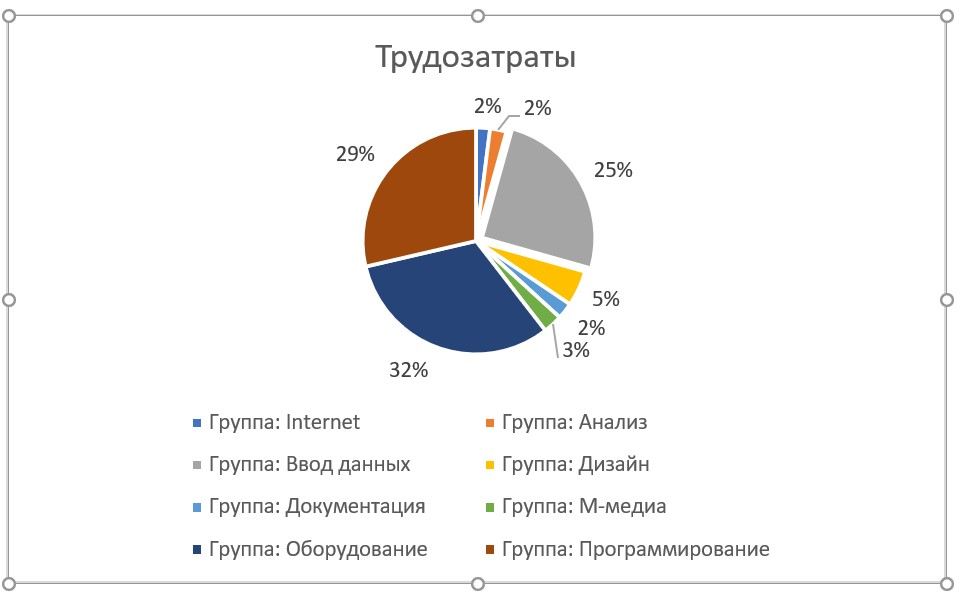
\includegraphics[width=0.9\textwidth]{img/task3/screen5.jpg}
	\caption{Диаграмма трудозатрат проекта}
	\label{fig:screen3_5}
\end{figure}

\begin{figure}[H]
	\centering
	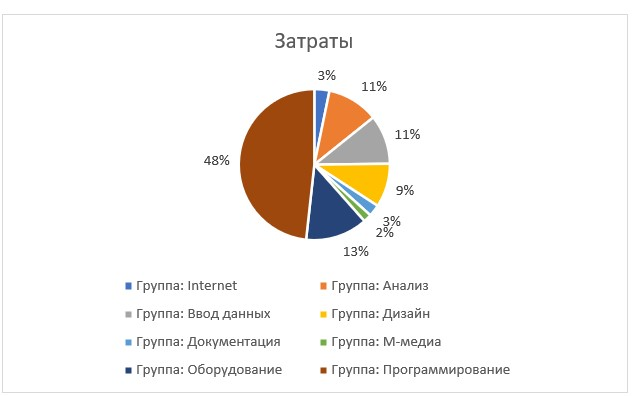
\includegraphics[width=0.9\textwidth]{img/task3/screen6.jpg}
	\caption{Диаграмма затрат проекта}
	\label{fig:screen3_6}
\end{figure}

По сравнению с лабораторной работой №2 затраты на программистов снизились на 2\% (с 50\% до 48\%), а на аналитика и технического писателя увеличились на 1\% (с 10\% до 11\% и с 2\% до 3\% соответственно).
Затраты на сервер выросли на 2 рубля и составили 6104 рубля.
Затраты на программистов снизились с 22580 рублей до 22172 рублей.
Затраты повысились из-за фиксированных трудозатрат, необходимых на выполнение задач и добавления 23 совещаний по 1 часу.
Проценты распределения трудозатрат не изменились, так как тип задач~---~фиксированные трудозатраты.

Затраты на программистов объясняются высокой квалификацией работников.
Их трудозатраты соотносятся с законом Брукса, то есть занимают 30\% времени работы.
Стоит задуматься о приобретении сервера вместо его аренды.
Группа <<Ввод данных>> (4850 рублей, 2400 часов) вносит существенный вклад в трудозатраты при сравнительно небольших затратах на ресурс.
Таким образом, можно для ускорения их работы нанять еще несколько наборщиков, так как это не сильно повлияет на затраты.
На аналитика тратится размер бюджета, несоразмерный объему работы, то есть распределение его времени работы на проекте необходимо оптимизировать.
Наименьший вклад в затраты и трудозатраты вносят ресурсы групп <<Internet>>, <<M-медиа>> и <<Документация>>.

Сохранение базового плана проекта продемонстрировано на рисунке~\ref{fig:screen3_8}.

\begin{figure}[H]
	\centering
	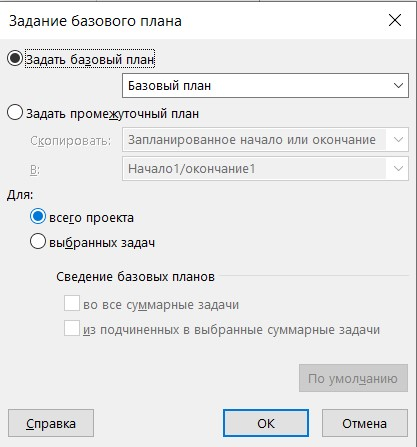
\includegraphics[width=0.9\textwidth]{img/task3/screen8.jpg}
	\caption{Сохранение базового плана проекта}
	\label{fig:screen3_8}
\end{figure}